\documentclass{report}
\usepackage{ctex}
\usepackage{geometry}
\usepackage{graphicx}
\usepackage{subfigure}
\usepackage{amsmath}
\usepackage{amssymb}
\usepackage{float}
\title{人工智能第二次实验实验报告}
\author{舒文炫}
\date{\today}
\geometry{a4paper,left=2cm,right=2cm,top=1cm,bottom=1cm}
\begin{document}
    \maketitle
    \tableofcontents
    \chapter{实验介绍}
    \section{实验内容}
    本次实验主要分为两个部分,第一部分为传统机器学习,第二部分为深度学习。
    \begin{itemize}
        \item 传统机器学习,包括实现线性分类器,多分类朴素贝叶斯以及支持向量机,使用的数据为鲍鱼数据集,助教已经做完了数据预处理,类别为三种,
        需要用这三种方法对数据分类
        \item 深度学习,分为实现多层感知机和复现MLP\_mixer,多层感知机数据为随机生成,主要考察实现前向传播,自动求导,反向传播,梯度下降。复现MLP\_mixer主要考察pytorch各种包的使用以及阅读文献的能力。
    \end{itemize}
    \section{实验环境}
    \begin{itemize}
        \item  虚拟环境Python3.6,不过实测在我原环境Python3.7也能运行(这主要是后面忘记在虚拟环境下运行,但是发现的时候并没有问题)
        \item  Pytorch版本:torch 1.9.0 torchvision 0.10.0
    \end{itemize}
    
    \chapter{实验设计}
    \section{part1:传统机器学习}
    线性分类器是考虑用线性模型$$Y=Xw+b+e$$拟合数据得出结果,这里X为数据,Y为数据类别标签,w,b为需要训练的参数,e是误差项,一般我们认为其为正态分布\par
    误差函数为$$L=\frac{1}{2n}(Xw-Y)^2+\frac{1}{2}\lambda w^2$$n为数据个数,$\lambda$为惩罚项,这一项的添加是防止出现共线性的情况,导致模型预测不准,如果使用回归分析里面岭回归的知识,可以直接求得闭式解 
    .在这里,我们运用梯度下降法求解,默认参数学习率lr=0.05,迭代1000次,$\lambda=0.001$,在这个误差函数下
    ,梯度为$$dL=\frac{1}{n}(X^TXw-X^TY)+\lambda w$$梯度下降法,每次向负梯度方向更新w为$w-lr*dL$,在学习率取的适当的情况下,
    可以保证损失函数递减,损失函数越小,这个模型在训练集上表现越好。预测则使用训练出的模型在测试集上判断类别,这里要分类,考虑分到每一个类别是的
    损失,我们取损失最小类别的为预测结果\par 
    朴素贝叶斯考虑用概率模型训练数据,主要用到贝叶斯公式,最简单的情况是$$P(A|B)=\frac{P(B|A)P(A)}{P(B|A)P(A)+P(B|A^C)P(A^C)}$$,这个公式使得我们在得到每个类别的出现概率,已经在该类别下,每个特征出现的概率之后,
    可以预测出已知这些特征的情况后,该数据类别是哪一类的概率。故我们的训练,即通过训练数据,给出训练数据的每个类别的概率,由于我们假设各个特征是在给的类别条件独立的
    故我们只要得到每个特征在每一类下的概率即可。同时考虑到泛化性能,对离散数据使用了拉普拉斯平滑,这个保证了,即使在测试集该特征出现了训练集没有的情况,也能处理。对连续数据,我假设其为正态分布,使用极大似然估计,求出该分布期望和方差的估计,用这个
    作为连续数据的分布。期望的极大似然估计为样本均值,方差的极大似然估计为$\frac{n-1}{n}Var(x)$,不过这不是无偏估计,一般在大样本下我们直接用样本方差来估计分布方差。
    最后的概率即将这些乘起来,但是考虑到精度问题,概率一般很小,乘起来结果在python里面可能为0.我们对每一项
    取了对数,再相加,这是考虑到有$\log(xy)=\log(x)+\log(y)$.预测即用我们得出的条件概率计算,概率最高值对应类别为预测类别。\par 
    SVM是考虑用一个分离超平面来分类数据,如果数据线性可分,SVM的准确率可以很高,可以达到百分之百,这里数据不一定会线性可分,我们要实现的是有软间隔的,即允许一些数据跨过分隔超平面。
    原型的SVM往往在实现时比较困难,这里我们采用其对偶形式,并使用核方法,实现了线性核,高斯核以及多项式核。考虑到会有精度问题,对很小的参数,我们直接置为0,即不将它对应的数据视为支持向量。
    对偶形式如下:

    \begin{gather*}
        min \frac{1}{2}\sum_{i=1}^N\sum_{j=1}^{N}\alpha_i\alpha_jy_iy_jK(x_i,x_j)+\sum_{i=1}^{N}\alpha_{i} \\
        s.t. \sum_{i=1}^{N}\alpha_iy_i=0 \\
        0 \leq \alpha_i \leq C\\
        i=1,2,3,...,N
    \end{gather*}
    其中$K(x_i,x_j)$为第i个和第j个数据算出的核,我们会得到一个N*N的核矩阵,$\alpha_i$为我们需要求的参数,C为惩罚参数,C越大,对误分类的惩罚越大。由上形式可知,此为一个关于$\alpha$的约束二次规划问题
    。\par 
    \section{part2:深度学习}
    深度学习这一块本身没有太多理论支撑,不过却有很好的结果,我觉得这很值得去探索。\par 
    MLP即多层感知机,是最简单的神经网络形式,分为输入层,隐含层,输出层,这里我们要实现一个四层的感知机,每层节点为5,4,4,3,其中5为输入层,两个隐含层
    节点个数为4,一个输出层节点个数为3.层与层直接采用全连接的形式,即通过一个线性变换,然后隐含层之间使用sigmoid激活函数,这样才能拟合数据非线性的情形,如果没有这个激活函数,无论
    使用多少层,所能拟合的也只有线性。这里我还准备加入额外的偏倚项,实验文档里面没有提到这个,感觉加入偏倚项可以使模型更鲁棒。隐含层与输出层之间使用softmax函数连接。这个函数可以将输出的结果转为概率分布,
    即输出的三个数和为1.这样方便使用交叉熵损失函数。然后还要实现反向传播,需要自己手动实现自动求导与torch的自动求导进行比较,用矩阵运算实现求导的公式在实验文档里面有描述,我在此不多赘述,比较容易实现。
    最后输出loss曲线,看是否实现了梯度下降,这里需要调用python画图的包,将每次迭代的loss储存起来,最后绘制。\par 
    MLP\_mixer是谷歌提出的一套框架,只使用最简单的MLP就能是模型达到特别高的精度,阅读文献后总结出,要复现这个模型,最重要的构建Mixer Layer.整个的大体框架为,先将图片拆成多个patch,然后用一个全连接网络对所有patch处理,
    提取出tokens,之后就要用到mixer layer层,(这里深度可以自行设计,要求是大于1)将特征信息不断提炼,最后通过一个全连接层输出结果进行预测。mixer分为token-mixer以及channel-mixer,简单来说就是分别对输入特征平面进行(1)沿列方向的特征提炼,
    (2)沿行方向的特征提炼。对MLP全连接层之间使用GELU激活函数。这一部分可以调用所有torch的包,实现起来代码比较精炼,主要是对框架的认识。\par 

    \chapter{实验实现}
    下面我将展示我的代码来解释具体实现:
    \section{part1:传统机器学习}
    \subsection{线性分类器}
    \begin{figure}[H]
        \centering
        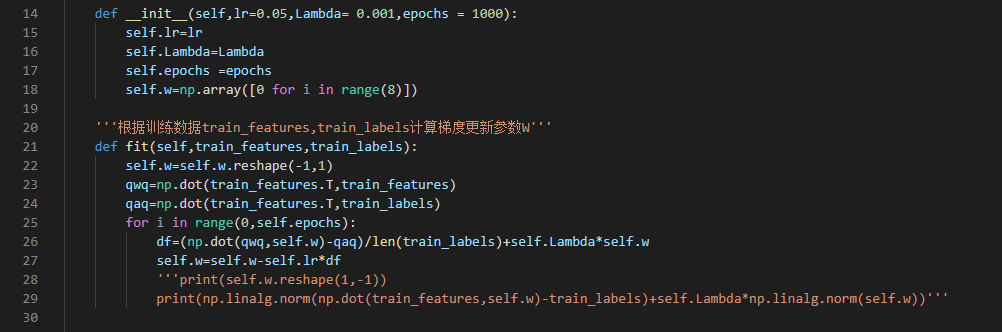
\includegraphics[width=15cm]{1.png}
        \caption{linearclassification fit}
    \end{figure}
    这里创建一个LinearClassfication类,init方法里面助教并没有给出参数w的初始化,这在fit训练w时将结果传给predict有点麻烦,故我在此添加了w的初始化.
    这对于这个类也是合理的,因为我们的模型就是要得到w,需要将其保存起来。
    在fit方法里面,为防止重复计算,我将$X^TX,X^TY$的值分别用qwq与qaq保存了起来,后面可以直接使用,第25到27行用for循环实现了梯度下降,迭代self.epochs次。
    梯度如前面实验设计里面所示。\par 
    \begin{figure}[H]
        \centering
        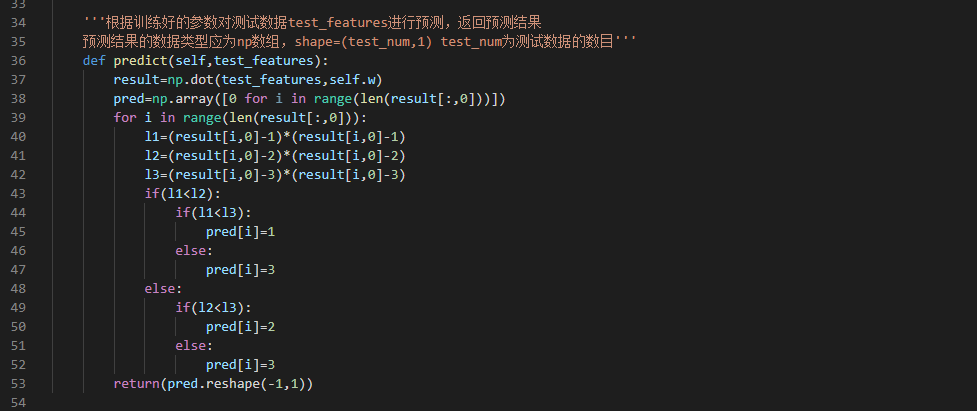
\includegraphics[width=15cm]{2.png}
        \caption{linearclassification predict}
    \end{figure}
    在这个predict方法里面,第37行用训练到的w在测试机算出每个数据的结果,但这个结果显然不会是1,2,3这样的离散值,故我在后面使用loss函数判断,
    如果分到某一类的loss函数最小,我就将其分到这一类,但是考虑到loss函数中有很多相等的常量,比如惩罚项,在给定了w后就都一样了。最重要的项就是计算预测结果到类别的距离这一项,故我只保留了该项,简化计算。
    39到52行用循环,一个一个分类,分类主要写了一个判断大小模块,l1,l2,l3分别表示到1,2,3的距离,选择距离最小的分到该类。\par 
    \subsection{多分类朴素贝叶斯}
    \begin{figure}[H]
        \centering
        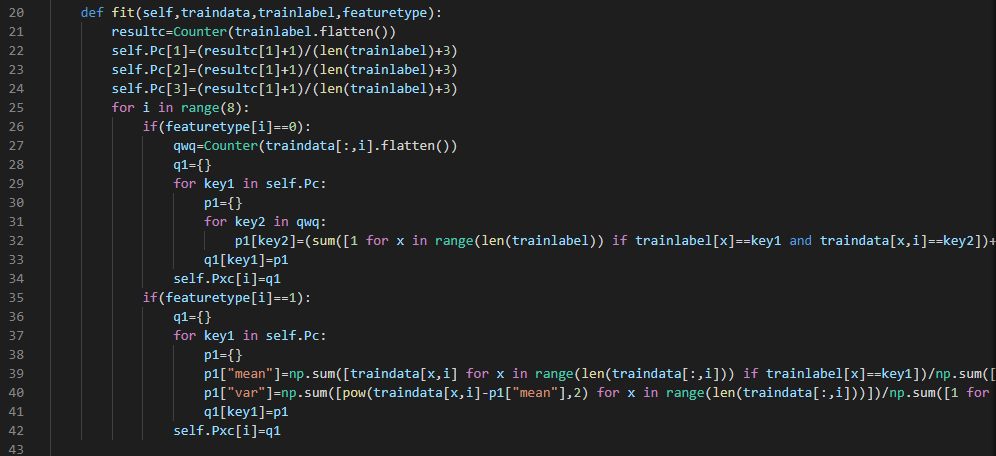
\includegraphics[width=15cm]{3.png}
        \caption{nbayes fit}
    \end{figure}
    这里某些行代码写的比较长,截不全,完整的可以直接看源代码。这个fit方法里面,我们先用counter方法,统计每个类别的个数,保存的数据类型类似字典,然后计算每个类别出现的概率,
    存到Pc字典里面。

    后面对每个feature,通过featuretype来区分时离散型还是连续型,离散型featuretype=0,此时使用拉普拉斯光滑,将结果存入Pxc字典中,这里储存是Pxc\{q1\{"1","2","3"\}\}两个字典嵌套,q1是该feature对应的字典,里面1,2,3对应储存了该feature在每个类别之中的概率
    ,对连续型featuretype=1,此时用正态分布去估计,同理也是存在Pxc字典里面,这个结构与离散型稍有不同,Pxc\{q1\{"mean","var"\}\},q1也是储存了对应feature的字典,里面由于是连续型,只需要保存均值和方差即可。
    \begin{figure}[H]
        \centering
        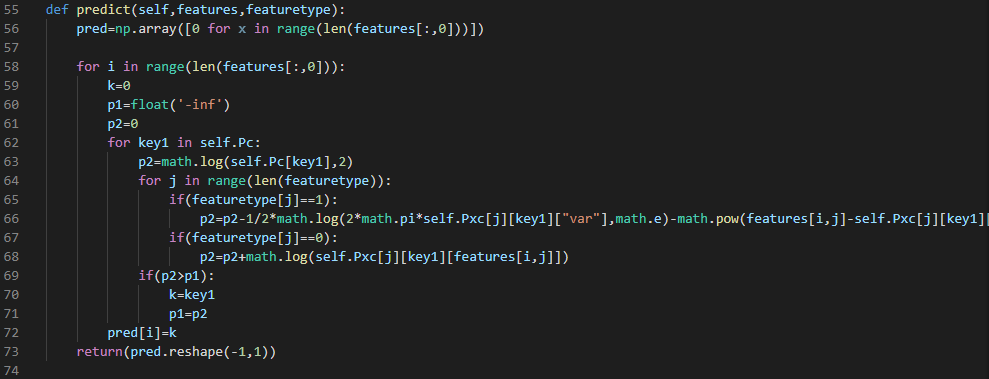
\includegraphics[width=15cm]{4.png}
        \caption{nbayes predict}
    \end{figure}
    这个predict方法,我先初始化了一个pred数组,用来储存预测出来的类别,后面一个for循环,对每组数据我们去计算这个数据在拥有对应特征下在每个类别里面的概率,去找最大值,
    这里我就直接用k暂时储存最大概率类别的类别,p1为最大的概率,p2为当前类别的概率。计算概率是取过了log的值,具体原因在实验设计里面说过了。\par 
    \subsection{SVM}
    \begin{figure}[H]
        \centering
        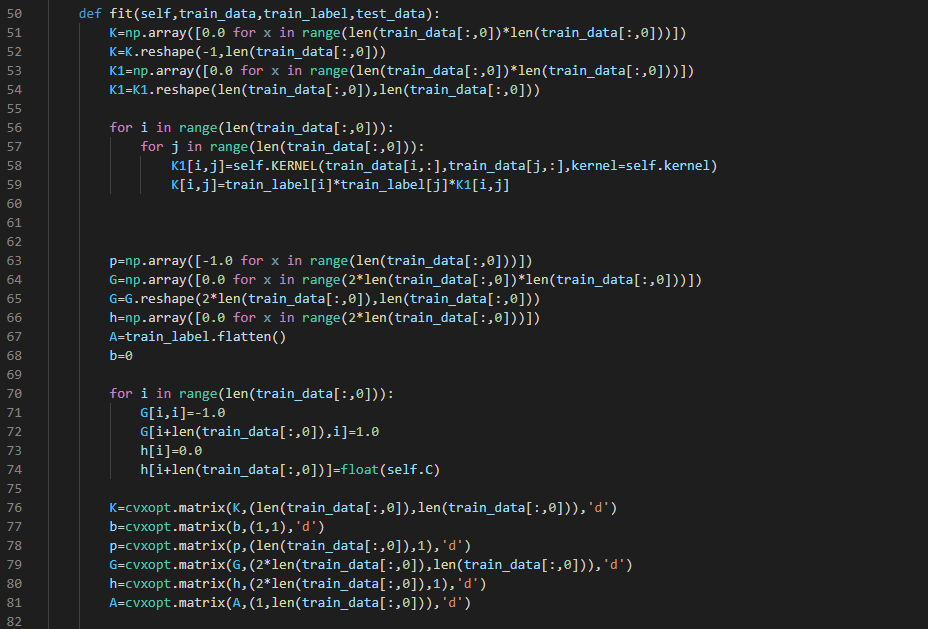
\includegraphics[width=15cm]{5.png}
        \caption{SVM 1}
    \end{figure}
    SVM只需要实现fit方法,不过里面的函数返回值就是预测类别。由于使用核方法,需要将这个核矩阵储存起来这里我使用K1来储存它,这里的K矩阵维数与K1一样,元素是K1对应元素乘上对应label,是为了简化后面的代码创建的。
    这里由于是求解二次规划问题,调用了cvxopt包,使用了cvxopt.solvers.qp(Q,p,G,h,A,b)函数。对应二次规划问题
    \begin{gather}
        min\  \frac{1}{2}x^TQx+px\\
        s.t. Gx \leq h \\
            Ax=b
    \end{gather}
    那么对应到这里,若记数据个数为n,Q=K,p为全为-1的向量,维数为n,G的话由于约束问题对每个$\alpha$两边都有约束,G的行数为2n,列数为n。前n行与后n行都是一个n维单位阵,h前n行为0,后n行为C。
    约束里面的等式约束为$\sum_{i=1}^{N}\alpha_iy_i=0$,所以转化为A为数据的标签,b为0,然后比较搞的一点,直接用numpy还不行,所以后面我将numpy转为了cvxopt里面的矩阵。
    \begin{figure}[H]
        \centering
        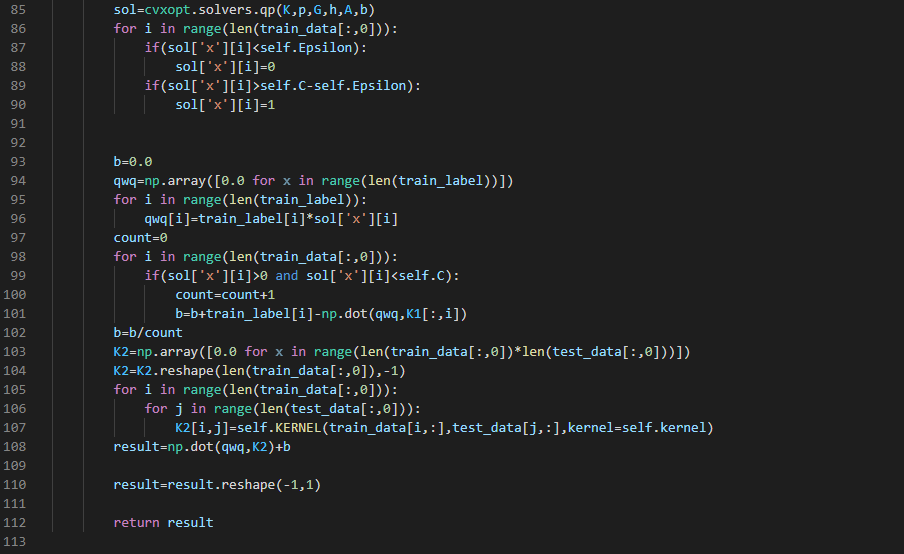
\includegraphics[width=15cm]{6.png}
        \caption{SVM 1}
    \end{figure}
    解出来的结果,我们还要处理一下,将过于接近0的$\alpha$去掉,和过于接近C的$\alpha$都置为C,这步是因为python自身的精度问题,过于小的数和接近C的数,最好是不视为支持向量,之前没有考虑这点,得出的准确度很低。
    后面的部分就是在测试集上预测了,我们使用公式
    \begin{align}
        w^*&=\sum_{i=1}^N\alpha^*_iy_ix_i\\
        b^*&=y_j-\sum_{i=1}^Ny_i\alpha_iK(x_i,x_j)
    \end{align}
    其中$\alpha^*_i$为二次规划的解,且第j个元素满足$0< \alpha_j < C$,即表明第j个为支持向量,当然若考虑鲁棒性,我们可以使用所以支持向量算出来的平均值,不考虑的话,这里用一个支持向量也没有大问题。
    qwq是我为了方便创建的一个数组,就是除掉核以外的那些系数,后面要预测,在测试集上我们需要算出新的核矩阵,记为K2,用这个和qwq点积即可。最后调整一下结果的维数,变成列向量输出。
    \section{part2:深度学习}

    \subsection{MLP manual}
    \begin{figure}[H]
        \centering
        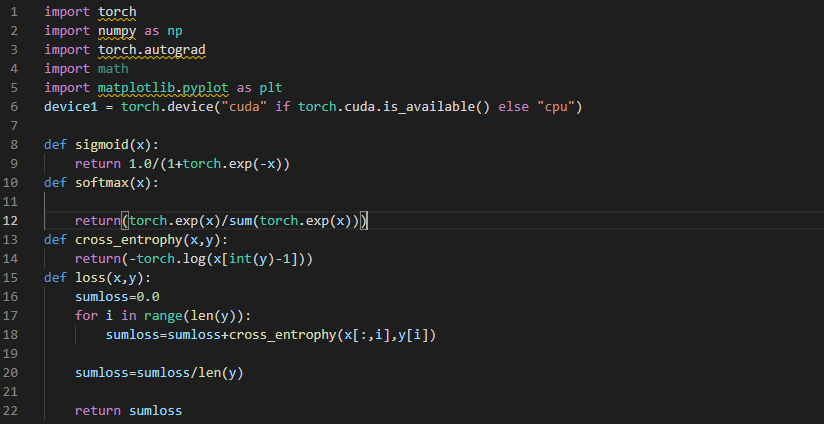
\includegraphics[width=15cm]{7.png}
        \caption{mlp 1}
    \end{figure}
    这一模块是我调用的包,只用到了基本的torch,以及需要比较自动求导与我手动实现,调用了torch.autograd。然后matplotlib.pyplot用于loss曲线
    的绘制,我安装了cuda,所以这个计算全都在GPU上运行,后面的sigmoid,softmax就是自己实现的对应的激活函数,其中交叉熵这里,我做了一点简化,考虑到如果用one-hot
    形式输入,在后面手动求梯度时还要去转为1,2,3这三类,比较麻烦。我就之间将y作为一个100维的列向量输入进去了(实验文档里也只说了输入lable为100维列向量,真转化为one-hot也不复杂,前面机器学习部分的代码里面就有),
    毕竟这种情况下的交叉熵其实也就是对对应的类别的值取负对数即可。然后loss函数就是对每组数据求交叉熵后求和的平均值。\par 
    \begin{figure}[H]
        \centering
        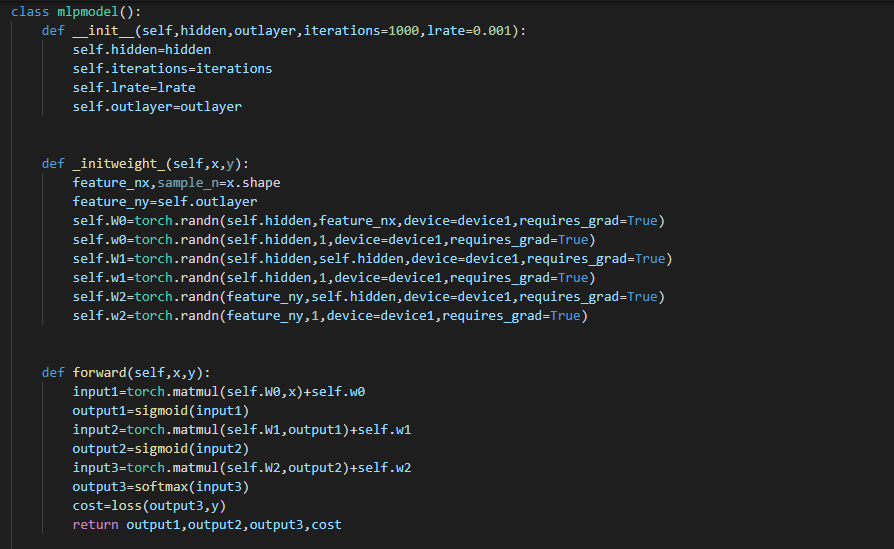
\includegraphics[width=15cm]{8.png}
        \caption{mlp 2}
    \end{figure}
    这里init方法里面,我定义了hidden为隐含层的节点数,lrate为每次梯度下降的学习率,outlayer为输出层的节点数,iteration为迭代次数,是这个网络最基本的构成
    ,故我单独列出来。后面initweight方法,是对权值矩阵的初始化,这一块比较多,为了方便阅读,没有直接放在init里面。这里权值矩阵的维数为(4*5),(4*4),(4*3).权值的初始化我用正态分布随机,w0,w1,w2为我加的三个偏倚量。
    这是因为如果全随机成0,经过测试比较奇怪,loss曲线基本是不动的,虽然这个不会影响求导。后面requires\_grad=True这个参数设置是为了后面与自动求导比较。\par 
    在forward方法,即正向传播里面,就依次对输入进行线性变换,激活这样操作,最后返回每一次激活后的输出以及cost,为自动求导和画loss曲线做准备。
    \begin{figure}[H]
        \centering
        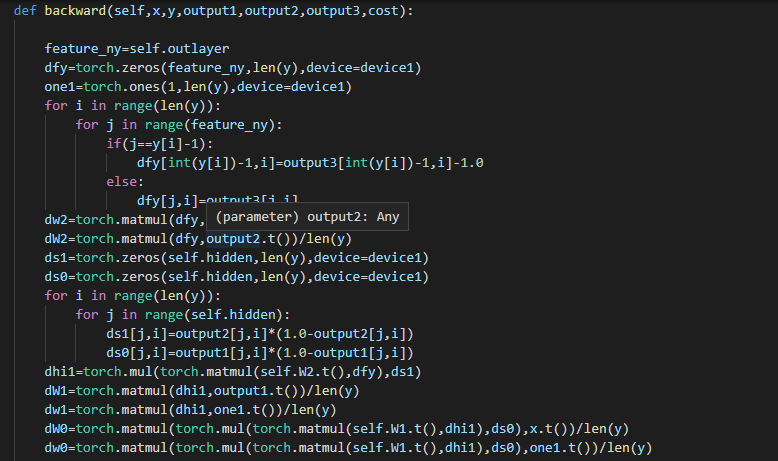
\includegraphics[width=15cm]{9.png}
        \caption{mlp back 1}
    \end{figure}
    这里开始反向传播,这部分分为两个小块,这里展示的是我手动用矩阵运算求导,公式都在助教给的实验文档里面写了,其中dfy矩阵是实验文档中对应的$(l's_3')$.
    dhi1矩阵是实验文档对应的$(W_3^T(l's_3')\odot s_2')$,(注意:我的代码里面,权值矩阵的编号是从0开始的),保存这两个值,主要是在矩阵运算中会反复用到,
    可以简化一下代码。最后每一个梯度的输出,我都是在对应的矩阵或向量前面加一个d表示。\par 
    \begin{figure}[H]
        \centering
        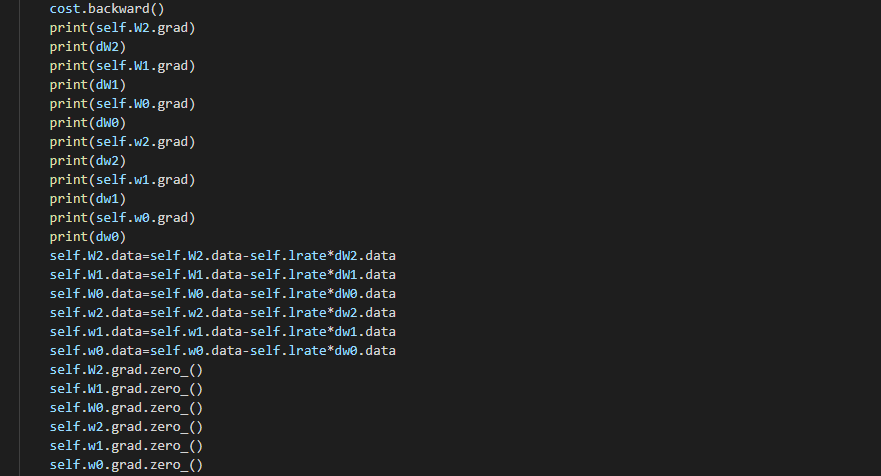
\includegraphics[width=15cm]{10.png}
        \caption{mlp back 2}
    \end{figure}
    这一块就是验证我的矩阵求导是否正确,输出是上面为torch自动求导的输出,下面为我手动求导的输出。每一步迭代这12个输出都会被打印出来,供比较。因为这里调用了torch的backward,
    原来的张量W0,W1,W2,w0,w1,w2已经被改动了,所以要在每个张量后面加上data表示用的是这个张量的值。梯度下降我用的是我自己求出来的梯度。后面是将梯度清零,这一步不做后面的梯度是错误的,会不断累积起来。\par 
    \begin{figure}[H]
        \centering
        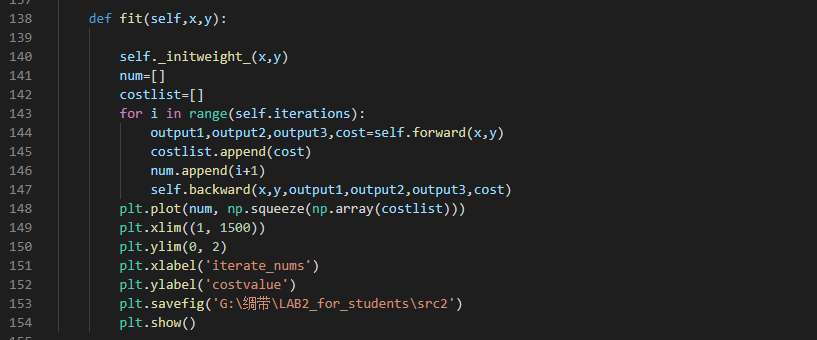
\includegraphics[width=15cm]{11.png}
        \caption{mlp fit}
    \end{figure}
    fit这一模块就是进行梯度下降,初始了两个列表,num和costlist用来保存迭代次数已经对应次数的loss,这个后面绘图时会用到。143行到147行就是不停的正向传播再反向传播。
    最后给出了一个结果plt.show方法将其展示出来。\par 
    \begin{figure}[H]
        \centering
        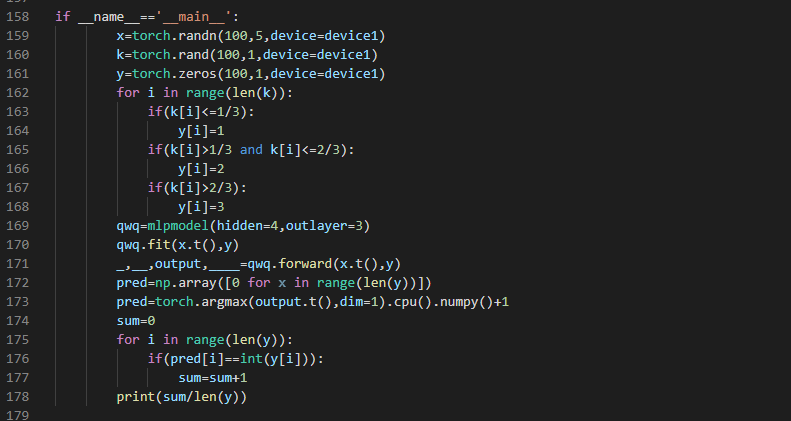
\includegraphics[width=15cm]{12.png}
        \caption{mlp main}
    \end{figure}
    这里主模块,我用正态分布随机生成100个五维的数据,以及(0,1)均匀分布100个1维标签,不过这里的标签是连续值,所以我后面处理了一下将(0,1)区间平均分为三段,每一段
    对应一个类别。后面调用我的mlp类训练出模型,pred是在训练集上预测结果,简单求了一下准确率(不过这里这步倒是没有太大必要)\par 
    
    \subsection{MLPmixer}
    \begin{figure}[H]
        \centering
        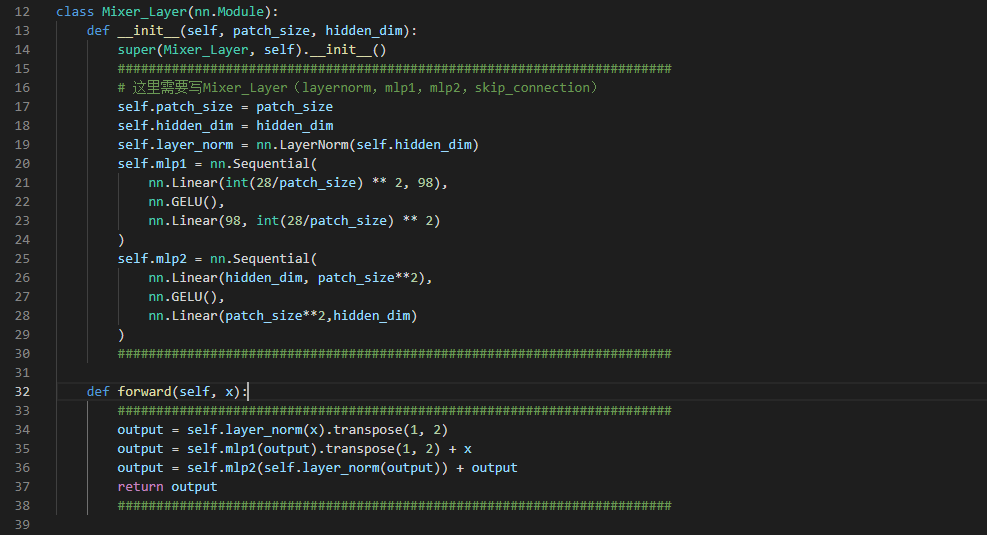
\includegraphics[width=15cm]{13.png}
        \caption{MLPmixer mixerlayer}
    \end{figure}
    这一块是mixer层,要求实现layernorm,mlp1,mlp2,skip connection。layernorm即做一个归一化,这在torch的包里面可以直接调用,这里layernorm的输入的最后一维是hidden\_dim维的所以参数用hidden\_dim,做归一化后需要进行转置,这里需要对特定的
    后面两维转置,这里用了transpose方法,可以指定将某两维转置。mlp1,mlp2对应的是
    文献中提到的那两个mlp层分别称为,token-mixing和channal-mixing,其中我直接用nn.linear做连接,mlp1层每一个数据输入为patchnum维即$(28/patchsize)^2$,中间的输出维数理论上没有要求,我直接就用patchnum维输出,只要最后面的linear保证输出维数和输入维数一样就行,mlp2层也是同理,保证输入和输出的维数相同,这里都是hidden\_dim维。
    两个linear中间是GELU激活函数,,这三个我用nn.sequential,按顺序包装在一起,显得紧凑。在forward里面,mlp1层的输出也是需要做了一个转置,然后做layernorm之后传给mlp2。skip connection的实现是在forward里面后面加上了x和output。
    skip connection就是直接拿上层的输入加入到输出里面,作用就是防止若网络比较深导致梯度爆炸或者梯度消失。\par 
    \begin{figure}[H]
        \centering
        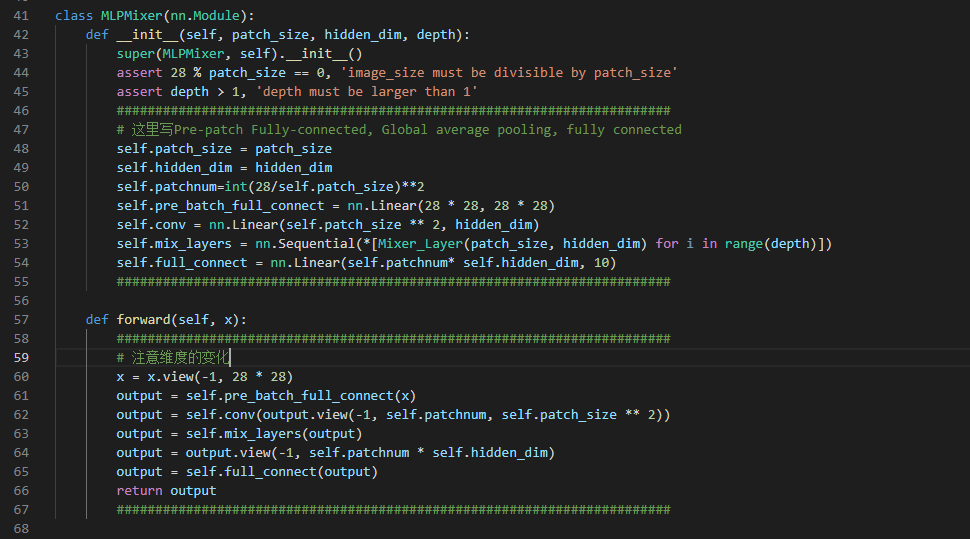
\includegraphics[width=15cm]{14.png}
        \caption{MLPmixer mlpmix}
    \end{figure}
    这一块就是mipmixer的框架,需要实现的Pre-patch Fully-connected, Global average pooling, fully connected如代码所示。Pre-patch Fully-connected嵌入层,即将图片由28*28展成1*(28*28)做一个全连接,这里用的
    linear。然后进行卷积,我们将一张图片拆成patchnum*$patchsize^2$,卷积之后得到每个patch整体的信息,得到三维的张量(datanum,patchnum,hidden\_dim),datanum是数据个数,patchnum是patch个数。
    将这个送入上面描述的mixer层,需要做depth个这样的mixer层,这里就直接用sequential简化了代码,sequential里面按顺序包装了depth个同样的mixer层。
    最后将结果通过一个全连接输出,输出维数(datanum,10),这里10是有10个类别。\par 
    \begin{figure}[H]
        \centering
        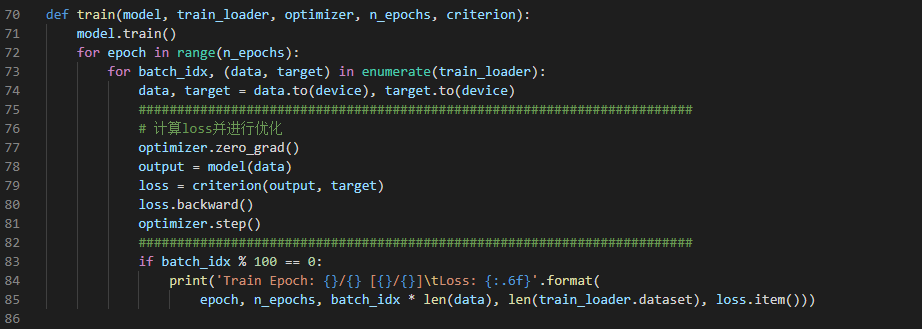
\includegraphics[width=15cm]{15.png}
        \caption{MLPmixer train}
    \end{figure}
    这里是train模块,每次train会传入一个batch数目的数据,每100次迭代就会输出一下。这里就调用optimizer对loss进行优化,loss函数用criterion函数进行计算,这里损失函数是交叉熵。\par 
    \begin{figure}[H]
        \centering
        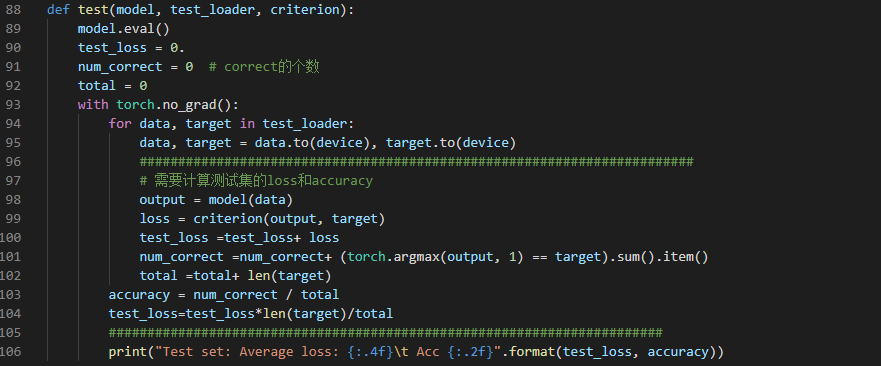
\includegraphics[width=15cm]{16.png}
        \caption{MLPmixer test}
    \end{figure}
    这里是test模块,将所有的测试集分批次导入到模型中,每次得到的loss相加,注意这里的loss是每个批次的平均loss,所有要求总的平均loss我们要将这个所有loss相加的结果乘以batchsize除以total,
    这里的batchsize可以由len(target)得到。这里的accuracy也是每次导入一批,我们将每个数的10个输出结果中最大的那个对应的类别视为预测类别。去和target比较,求和再将这个数提取出来,即为这一批的
    num\_correct,然后所有批次的相加即可。\par 








    \chapter{实验结果与分析}
    \section{part1:传统机器学习}
    这一部分我会贴上我的输出\par 
    \subsection{线性分类器}
    \begin{figure}[H]
        \centering
        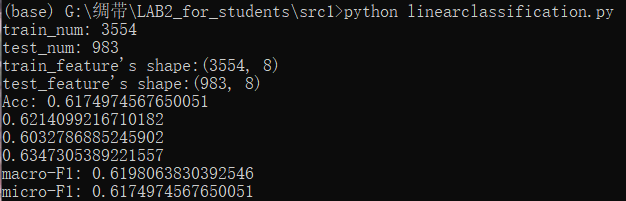
\includegraphics[width=15cm]{lc.png}
        \caption{linearclassification output}
    \end{figure}
    这是线性分类器的输出结果,可以看到总的预测准确度达到了0.61,对每个类别的准确度也有0.6朝上,micro-F1和macro-F1也有0.6以上,说明
    模型实现没有问题,结果比较理想\par 
    \subsection{多分类朴素贝叶斯}
    \begin{figure}[H]
        \centering
        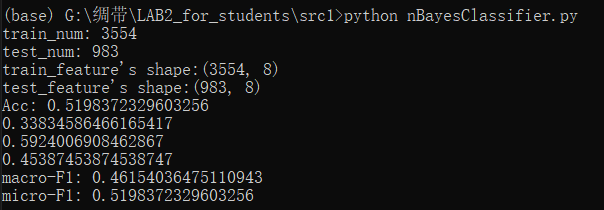
\includegraphics[width=15cm]{nb.png}
        \caption{nbayes output}
    \end{figure}
    这是朴素贝叶斯的输出结果,可以看到总的预测准确度达到0.5,比线性分类器稍差,也有可能还是精度有一定影响,或者假设为正态分布没有特别合理,但是结果也还可以。
    总体实现没有太大问题。
    \subsection{SVM}
    \begin{figure}[H]
        \centering
        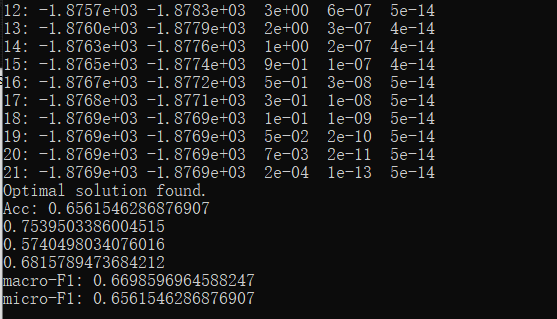
\includegraphics[width=15cm]{SVM_gauss3.png}
        \caption{SVM gauss output}
    \end{figure}
    \begin{figure}[H]
        \centering
        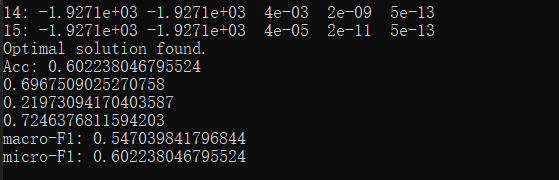
\includegraphics[width=15cm]{SVM_linear3.png}
        \caption{SVM linear output}
    \end{figure}
    \begin{figure}[H]
        \centering
        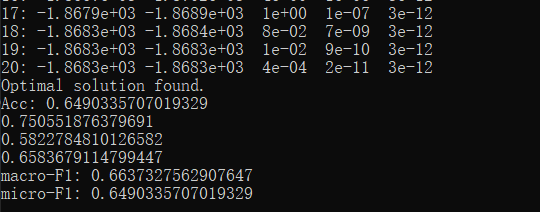
\includegraphics[width=15cm]{SVM_poly3.png}
        \caption{SVM poly output}
    \end{figure}
    这三张图分别是选择高斯核,线性核,多项式核的结果,前面是二次规划迭代过程,很长就没有一一截下来,截下来也没有太大意义,可以看到高斯核准确率0.65,各个类别的f1-score也很不错,线性核低一点只有0.60,多项式核准确率0.64,比线性核好,
    比高斯核差一点。总体而言这三种核的准确率都很好,所以SVM实现也没有问题。

    \section{part2:深度学习}
    \subsection{MLP manual}
    \begin{figure}[H]
        \centering
        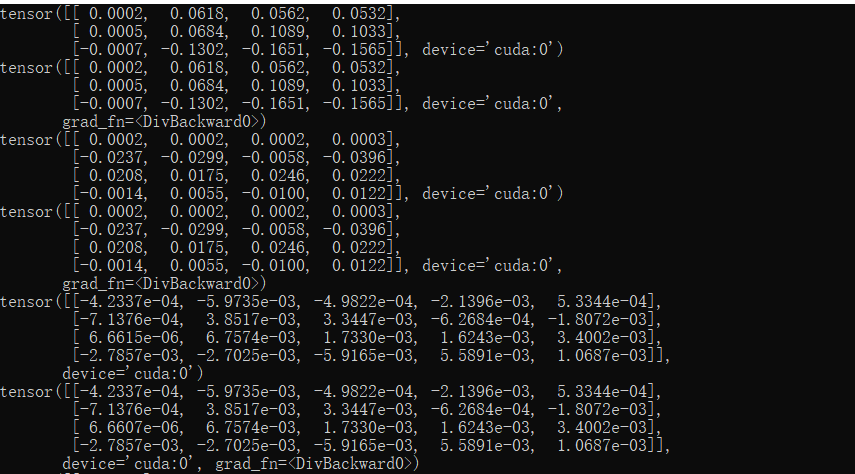
\includegraphics[width=15cm]{MLP1.png}
        \caption{mlp output1}
    \end{figure}
    \begin{figure}[H]
        \centering
        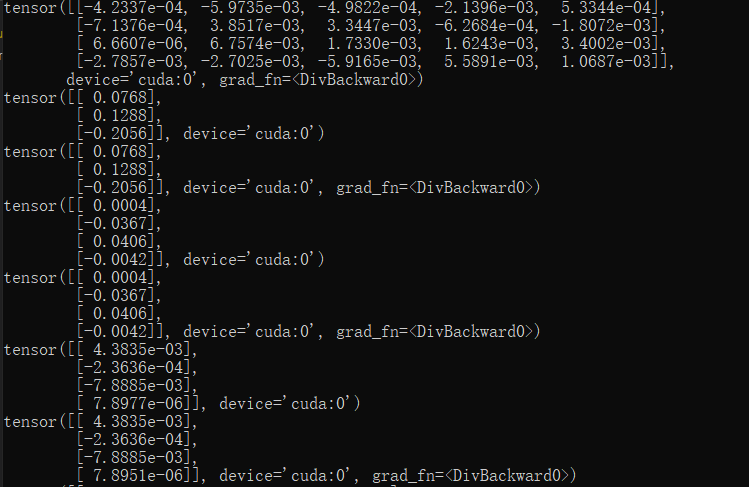
\includegraphics[width=15cm]{MLP2.png}
        \caption{mlp output2}
    \end{figure}
    这一个输出是检验手动求导和自动求导是否相同。我迭代了1000次,这里输出有很多,我只随机截取其中一组输出。每一组有12个输出,其中连续两个输出进行比较,对应W2,W1,W0,w2,w1,w0
    上面的为自动求导的参数,下面为手动求导参数,可以看到,这个是相同的,助教也可以自行查看其它的,都是相同的。手动 求导的实现是没有问题的。\par 
    \begin{figure}[H]
        \centering
        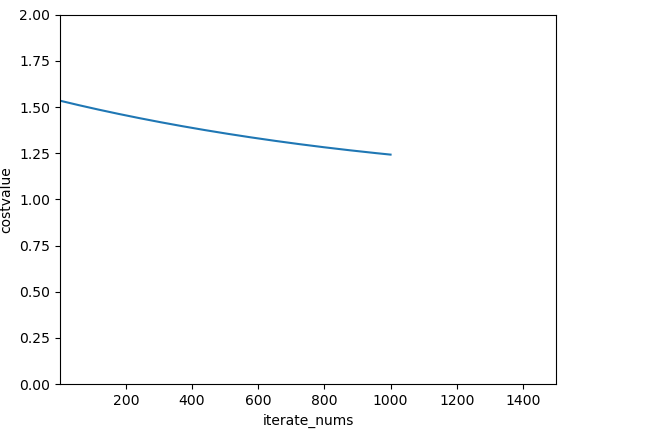
\includegraphics[width=15cm]{MLPloss.png}
        \caption{mlp output3}
    \end{figure}
    这个图就是loss曲线,可以看到这个曲线是下降趋势的,不过由于数据随机,这个loss比较高。这个梯度下降的实现是没有问题的。\par
    \subsection{MLPmixer}
    \begin{figure}[H]
        \centering
        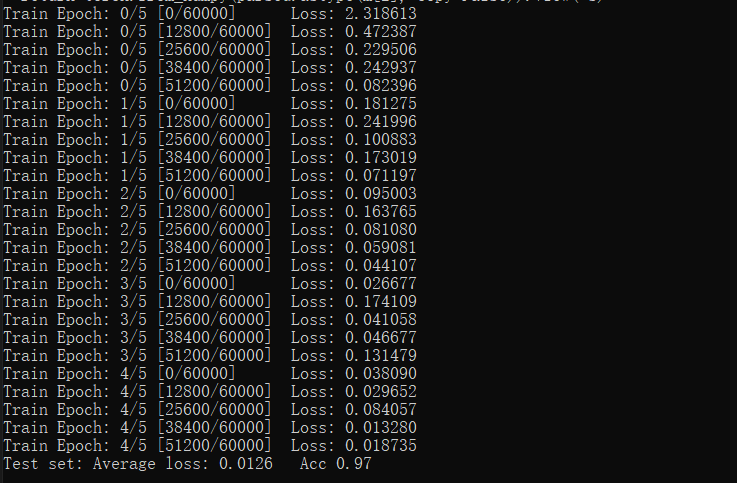
\includegraphics[width=15cm]{mlpmixer.png}
        \caption{mlpmixer}
    \end{figure}
    这个图是我实现的MLPmixer的输出,可以看到在测试集上平均损失只有0.0126,准确率也达到了0.97,这说明我的实现也没有问题。\par 



    \chapter{实验总结}
    本次实验,我接触到了传统机器学习的各种经典方法,并尝试实现了他们,这让我对机器学习理解更为深刻,也初步接触了深度学习相关知识,体会到了深度学习比传统的
    机器学习的优越性,也锻炼了我查找资料的能力.






    

\end{document}